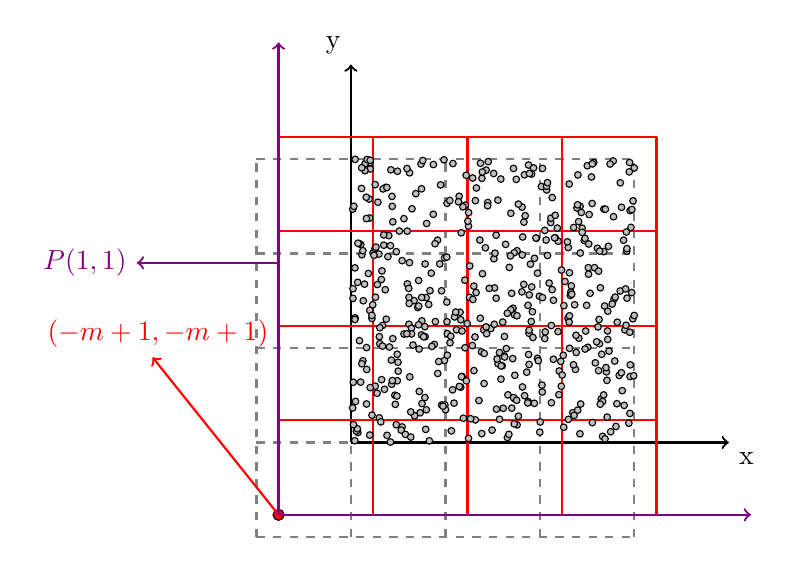
\begin{tikzpicture}[scale=0.4]

    % Draw the grid
    \draw[step=3cm,dashed, gray, thick] (0,0) grid (12,12);

    \draw[thick,->,black] (3,3) -- (15,3) node[anchor=north west] {x};
    \draw[thick,->,black] (3,3) -- (3,15) node[anchor=south east] {y};

    \begin{scope}[xshift = 20, yshift = 20]
    
    \filldraw[fill=red] circle (5pt) ;
        
    \draw[red, ->, thick] (0, 0) -- (-4, 5) node[above] {\textbf{ $(-m+1,-m+1)$}};

    \draw[step=3cm, red, thick] (0,0) grid (12,12);
    

    \draw[thick,->,violet] (0,0) -- (15,00) ;
    \draw[thick,->,violet] (0,0) -- (0,15) ;

    \draw[thick,->,violet] (0,8) -- (-4.5,8) node[left] {$P(1,1)$};

    \end{scope}

    % Seed for randomness
    \pgfmathsetseed{42}  % Set seed for reproducibility

    % Generate 10 random points within the grid
    \foreach \i in {1,...,500} {
        \pgfmathsetmacro{\x}{3 + rnd*9}
        \pgfmathsetmacro{\y}{3 + rnd*9}

        % \ifdim \x pt > 3pt \ifdim \x pt < 6pt \ifdim \y pt > 3pt \ifdim \y pt < 6pt
        %     \filldraw[fill=red] (\x,\y) circle (3pt); % Draw red point
        % \else
            \filldraw[fill=gray!50] (\x,\y) circle (3pt); % Draw gray point
        % \fi\fi\fi\else
        %     \filldraw[fill=gray!50] (\x,\y) circle (3pt); % Draw gray point
        % \fi
    }

\end{tikzpicture}